De acordo com o artigo \cite{langford08} e como dito no capítulo \ref{chap:nocoes_preliminares}, um classificador que apresente um erro $\alpha$ na acurácia, pode apresentar um erro teórico máximo de $\alpha \cdot n$, onde $n$ é a cardinalidade da base a ser ordenada. A técnica de \emph{ranking reduzido a classificação} diminui esse limite para $\alpha * 2$ usando o mesmo classificador com erro $\alpha$ na acurácia.

Quanto maior o desbalanceamento entre as classes da base a ser ordenada, maior a chance de intensificação do erro na ordenação. Partindo desse princípio, foi montada uma estratégia de testes com cinco bases de dados com diferentes níveis de desbalanceamento. Tais bases podem ser encontradas no repositório da University of California, Irvine (UCI)\footnote{http://archive.ics.uci.edu/ml/}.

\section{Características das bases}

As bases usadas foram as seguintes: Breast Cancer; Statlog (Vehicle Silhouettes), chamada de Vehicle; Hepatitis; Glass Identification, chamada de Glass e Yeast. Como o algoritmo proposto em {{langford}} tem um custo computacional alto, $O(n^2)$ para treinamento e $O(n^2)$ para gerar o ranking; isso aliado ao baixo controle sobre o ambiente de execução culminou na escolha de bases pequenas para avaliação do experimento.

As bases Vehicle, Glass e Yeast tratam, originalmente, de problemas multiclasse. A essas bases foram aplicadas transformações, descritas em \cite{guo04}, a fim de torná-las problemas de classe binária. Para as bases Vehicle e Glass, foram unidas todas as classes, exceto a minoritária, em uma nova classe. Para a base Yeast, apenas as classes de valor 'CYT' ou 'POX' foram consideradas.

Cada base utilizada apresenta diferenças em: desbalanceamento entre as classes, número de atributos, número de instâncias, entre outros. A tabela \ref{tbl:caracteristicas} mostra um resumo sobre as características das bases.

\begin{table}[h]

    \begin{tabular}{c c c c c c c}
        \hline
        \multirow{2}{*}{Bases} & \multicolumn{2}{c}{Atributos} & \multirow{2}{*}{Instâncias} & \multicolumn{3}{c}{Classe} \\ \cline{2-3} \cline{5-7}
        & {\small Contínuos} & {\small Discretos} & & {\small Minoritária} & {\small Majoritária} & {\small Distribuição}\\
        \hline
        breast-cancer & 0 & 9 & 286 & 85 & 201 & 30\% - 70\%\\
        vehicle & 18 & 0  & 846 & 199 & 647 & 23\% - 77\%\\
        hepatitis & 6 & 13  & 155 & 32 & 123 & 20\% - 80\%\\
        glass & 9 & 0  & 214 & 29 & 185 & 13\% - 87\%\\
        yeast & 8 & 0  & 483 & 20 & 463 & 4\% - 96\%\\
        \hline
    \end{tabular}

    \caption{Dados sobre as bases usadas para \emph{ranking}. \label{tbl:caracteristicas}}
\end{table}

\section{Execução e Avaliação do Algoritmo}
\label{sec:avaliacao}

Foram escolhidos quatro classificadores base para avaliar o algoritmo: J48, Naïve Bayes, Logistic e SMO. O motivo da escolha desses classificadores é o reconhecimento de tais como padrões em suas famílias, J48 para árvores de decisão (implanta a árvore de decisão C4.5), Naïve Bayes para estatísticos, Logistic (implanta curva logística) e SMO (implanta Support Vector Machine) para classificadores baseados em funções.

Para cada classificador base houve quatro baterias de execução com diferentes configurações:

\begin{enumerate}

    \item Somente o classificador;
    \item O classificador como base para a técnica de \emph{ranking reduzido a classificação} original;
    \item O classificador como base para o algoritmo de ranking com configurações de 1 par por instância e variando o número de classificadores na votação entre 1 e 20;
    \item O classificador como base para o algoritmo de ranking com configurações de 1 classificador na votação e variando o número de pares por instância entre 1 e 20.

\end{enumerate}

Nas três baterias que envolveram o algoritmo de \emph{ranking}, o método de ordenação usado para gerar o resultado final foi o \emph{torneio}, como explicado no artigo {{langford}}. Em todas as baterias foi executada uma validação cruzada com 10 partições e os resultados apresentados nas tabelas é a média das \emph{AUCs} obtidas para cada partição.

Para as tabelas de número \ref{j48_results_table}, \ref{nb_results_table}, \ref{logistic_results_table} e \ref{smo_results_table}; o símbolo \textbf{*} significa ranking aplicado com 1 par por instância e 10 classificadores na votação. O símbolo \textbf{**} significa ranking aplicado com 10 pares por instância e 1 classificador na votação.

\clearpage
\pagebreak

\subsection{Desempenho para \emph{C4.5} (trees.J48)}


\begin{table}[h!]
    \begin{tabular}{ c c c c c }
        \hline
    
        \multirow{2}{*}{Bases} & \multirow{2}{*}{J48} & \multicolumn{3}{c}{J48 acrescido de} \\ \cline{3-5}
        & & {\small Ranking Original} & {\small Ranking*} & {\small  Ranking**} \\

        \hline
        
        breast-cancer & {\small \textbf{0,62806 (0,01005)}} & {\small 0,46784 (0,03049)} & {\small 0,51289 (0,01950)} & {\small 0,45055 (0,02984)} \\
        vehicle & {\small 0,93725 (0,00056)} & {\small 0,91389 (0,00624)} & {\small \textbf{0.98072 (0.00017)}} & {\small 0,95670 (0,00071)} \\
        hepatitis & {\small 0,69655 (0,04084)} & {\small 0,67112 (0,03127)} & {\small \textbf{0,74322 (0,03925)}} & {\small 0,72179 (0,04571)} \\
        glass & {\small \textbf{0,90322 (0,01578)}} & {\small 0,83772 (0,03524)} & {\small 0,89016 (0,02934)} & {\small 0,88860 (0,02668)} \\
        yeast & {\small 0,48918 (0,00021)} & {\small \textbf{0,95009 (0,01453)}} & {\small 0,78550 (0,03630)} & {\small 0.84806 (0.01924)} \\
    
        \hline
    \end{tabular}
    
    \caption{Desempenho para árvore de decisão C4.5}
    \label{j48_results_table}
\end{table}

\begin{figure}[h!]
    \centering
    \subfloat[Breast cancer]{
        \label{fig:breast-cancer_j48}
        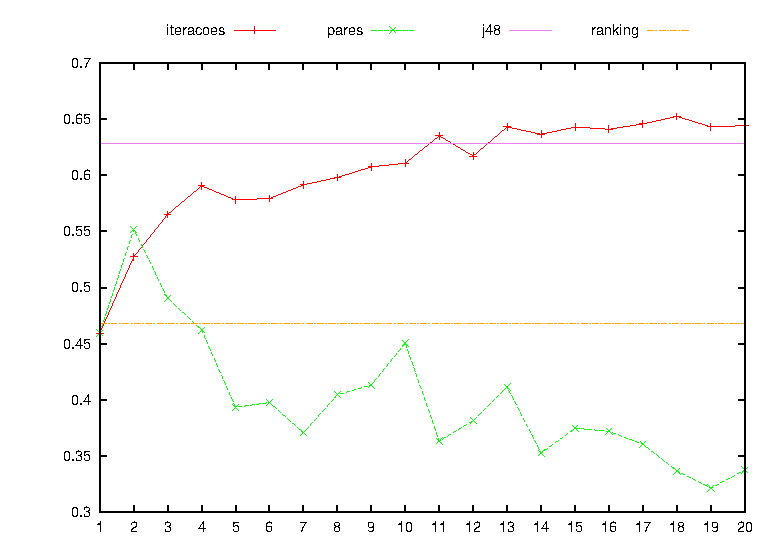
\includegraphics[width=0.42\textwidth]{img/breast-cancer_j48.eps}
    }
    \subfloat[Glass]{
        \label{fig:glass_j48}
        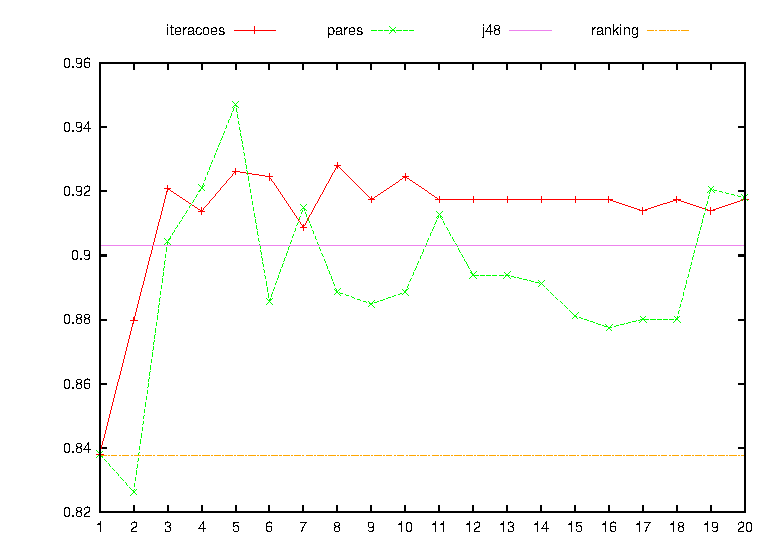
\includegraphics[width=0.42\textwidth]{img/glass_j48.eps}
    }

    \subfloat[Hepatitis]{
        \label{fig:hepatitis_j48}
        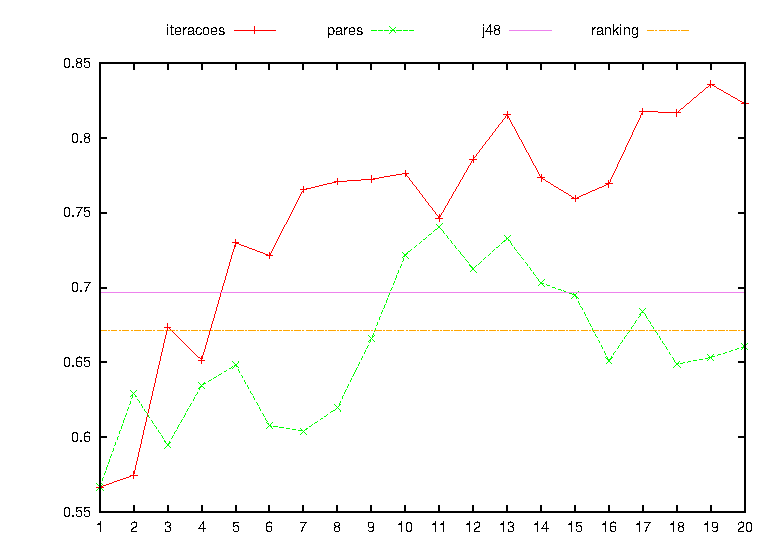
\includegraphics[width=0.42\textwidth]{img/hepatitis_j48.eps}
    }    
    \subfloat[Vehicle]{
        \label{fig:vehicle_j48}
        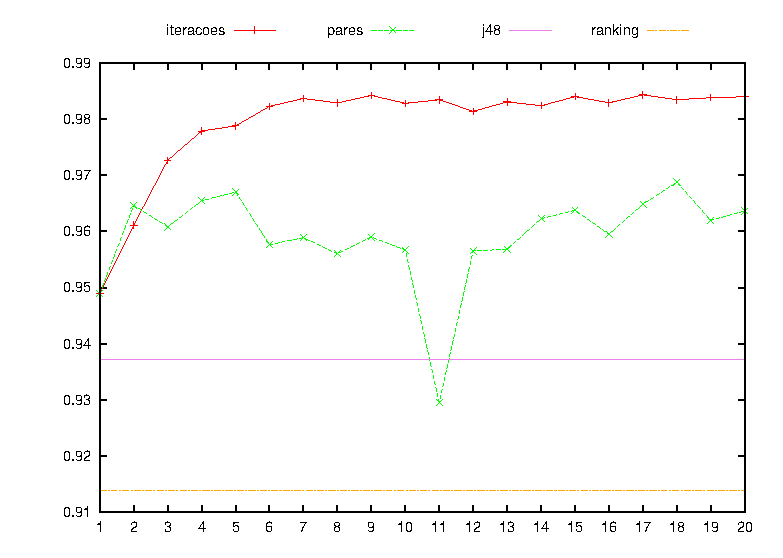
\includegraphics[width=0.42\textwidth]{img/vehicle_j48.eps}
    }

    \subfloat[Yeast]{
        \label{fig:yeast_j48}
        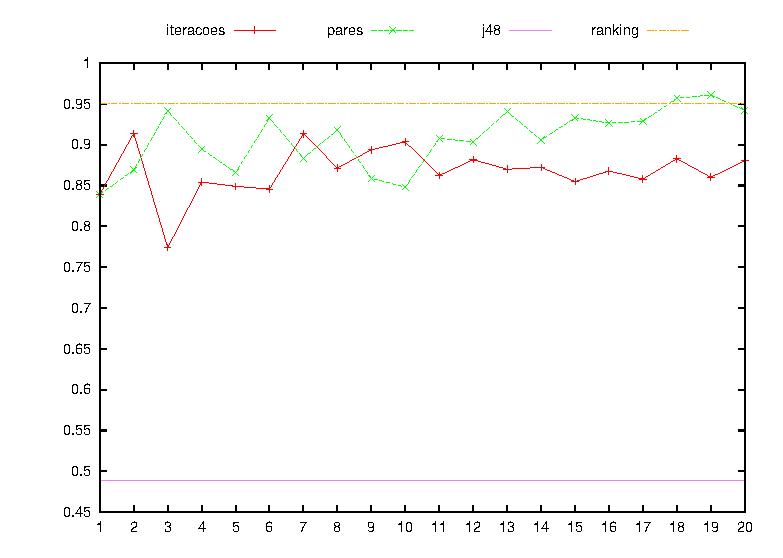
\includegraphics[width=0.42\textwidth]{img/yeast_j48.eps}
    }

    \caption{Gráficos de desempenho para árvore de decisão C4.5}
\end{figure}

\clearpage
\pagebreak


\subsection{Desempenho para \emph{Naïve Bayes} (bayes.NaiveBayes)}

\begin{table}[h!]
    \begin{tabular}{ c c c c c }
        \hline

        \multirow{2}{*}{Bases} & \multirow{2}{*}{Naïve Bayes} & \multicolumn{3}{c}{Naïve Bayes acrescido de} \\ \cline{3-5}
        & & {\small Ranking Original} & {\small Ranking*} & {\small  Ranking**} \\
    
        \hline
        
        breast-cancer & {\small \textbf{0,71543 (0,01899)}} & {\small 0,20857 (0,00620)} & {\small 0,04976 (0,00445)} & {\small 0,04532 (0,00426)} \\
        vehicle & {\small \textbf{0,80898 (0,00468)}} & {\small 0,24323 (0,01559)} & {\small 0,00310 (0,00004)} & {\small 0,12514 (0,01546)} \\
        hepatitis & {\small \textbf{0,85919 (0,01190)}} & {\small 0,22489 (0,05188)} & {\small 0,06052 (0,00265)} & {\small 0.06608 (0,00101)} \\
        glass & {\small \textbf{0,94084 (0,01099)}} & {\small 0,17271 (0,02416)} & {\small 0,02222 (0,00151)} & {\small 0,02476 (0,00132)} \\
        yeast & {\small 0,82863 (0.06355)} & {\small 0,84269 (0,03505)} & {\small \textbf{1,00000 (0,00000)}} & {\small \textbf{1,00000 (0,00000)}} \\
    
        \hline
    \end{tabular}
    
    \caption{Desempenho para Naïve Bayes}
    \label{nb_results_table}
\end{table}

\begin{figure}[h!]
    \centering
    \subfloat[Breast cancer]{
        \label{fig:breast-cancer_naive-bayes}
        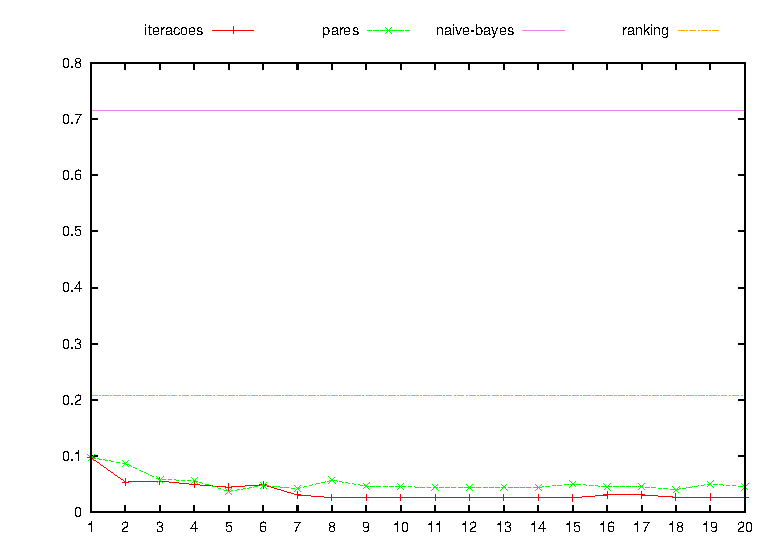
\includegraphics[width=0.42\textwidth]{img/breast-cancer_naive-bayes.eps}
    }
    \subfloat[Glass]{
        \label{fig:glass_naive-bayes}
        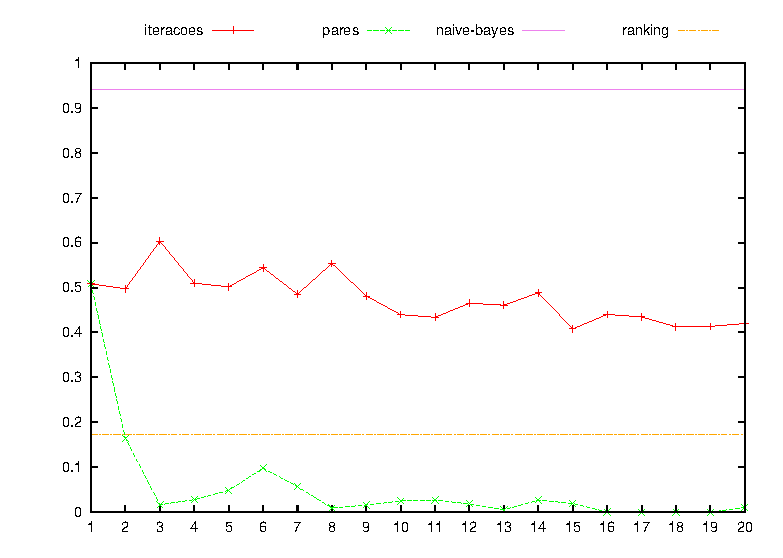
\includegraphics[width=0.42\textwidth]{img/glass_naive-bayes.eps}
    }

    \subfloat[Hepatitis]{
        \label{fig:hepatitis_naive-bayes}
        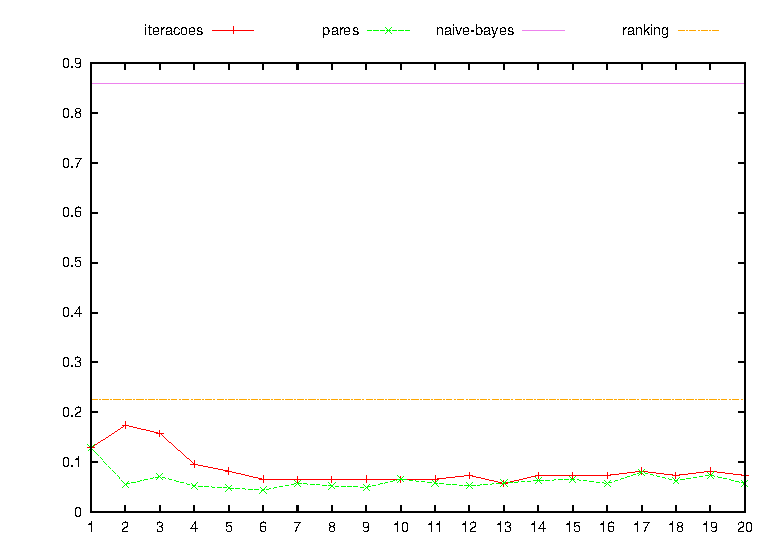
\includegraphics[width=0.42\textwidth]{img/hepatitis_naive-bayes.eps}
    }    
    \subfloat[Vehicle]{
        \label{fig:vehicle_naive-bayes}
        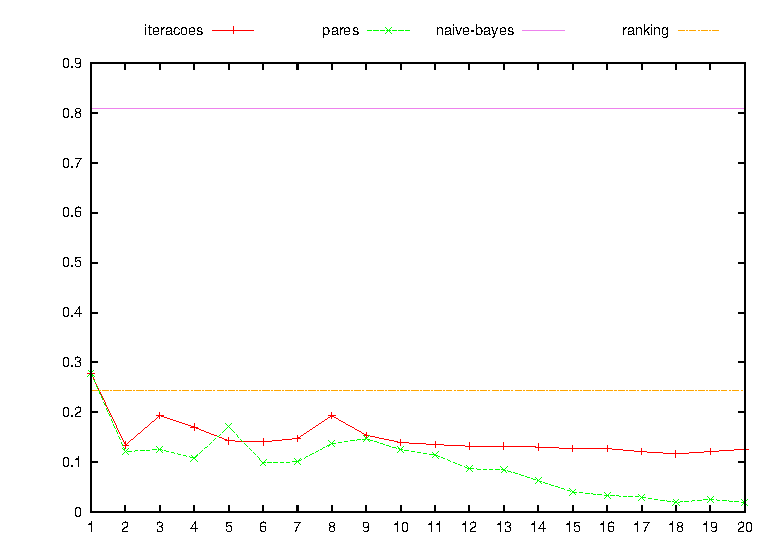
\includegraphics[width=0.42\textwidth]{img/vehicle_naive-bayes.eps}
    }

    \subfloat[Yeast]{
        \label{fig:yeast_naive-bayes}
        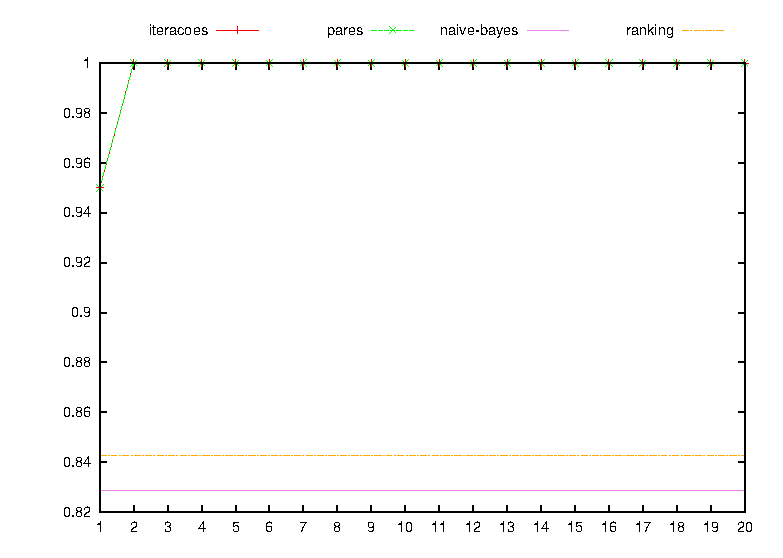
\includegraphics[width=0.42\textwidth]{img/yeast_naive-bayes.eps}
    }

    \caption{Gráficos de desempenho para Naïve Bayes}
\end{figure}

\clearpage
\pagebreak


\subsection{Desempenho para a \emph{Curva Logística} (functions.Logistic)}

\begin{table}[h!]
    \begin{tabular}{ c c c c c }
        \hline

        \multirow{2}{*}{Bases} & \multirow{2}{*}{Logistic} & \multicolumn{3}{c}{Logistic acrescido de} \\ \cline{3-5}
        & & {\small Ranking Original} & {\small Ranking*} & {\small  Ranking**} \\
        
        \hline
        
        breast-cancer & {\small 0,66625 (0,02322)} & {\small \textbf{0,66740 (0,02364)}} & {\small 0,65784 (0,02143)} & {\small 0,65132 (0,02219)} \\
        vehicle & {\small 0,99358 (0,00003)} & {\small \textbf{0,99420 (0,00003)}} & {\small 0,99358 (0,00003)} & {\small 0,99234 (0,00002)} \\
        hepatitis & {\small \textbf{0,80924 (0,02598)}} & {\small 0,79882 (0,02432)} & {\small 0,75064 (0,04278)} & {\small 0,74557 (0,05075)} \\
        glass & {\small 0,95965 (0,00308)} & {\small \textbf{0,97037 (0,00192)}} & {\small 0,96101 (0,00484)} & {\small 0,95536 (0,00384)} \\
        yeast & 0{\small ,85805 (0,04115)} & {\small 0,83453 (0,04931)} & {\small \textbf{0,87414 (0,03463)}} & {\small 0,85691 (0,03997)} \\
    
        \hline
    \end{tabular}
    
    \caption{Desempenho para Logistic}
    \label{logistic_results_table}
\end{table}

\begin{figure}[h!]
    \centering
    \subfloat[Breast cancer]{
        \label{fig:breast-cancer_logistic}
        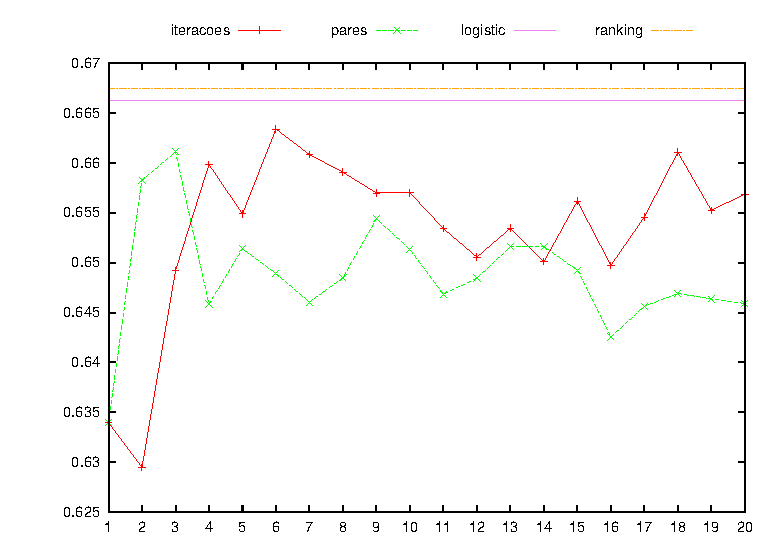
\includegraphics[width=0.42\textwidth]{img/breast-cancer_logistic.eps}
    }
    \subfloat[Glass]{
        \label{fig:glass_logistic}
        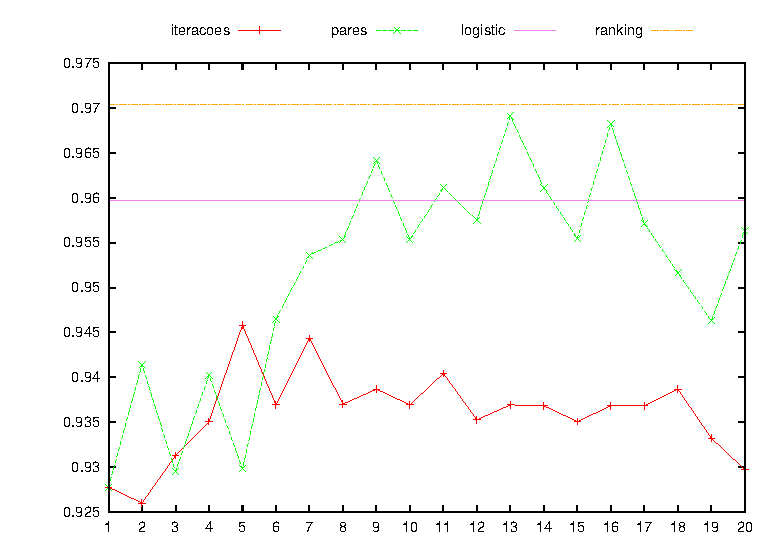
\includegraphics[width=0.42\textwidth]{img/glass_logistic.eps}
    }

    \subfloat[Hepatitis]{
        \label{fig:hepatitis_logistic}
        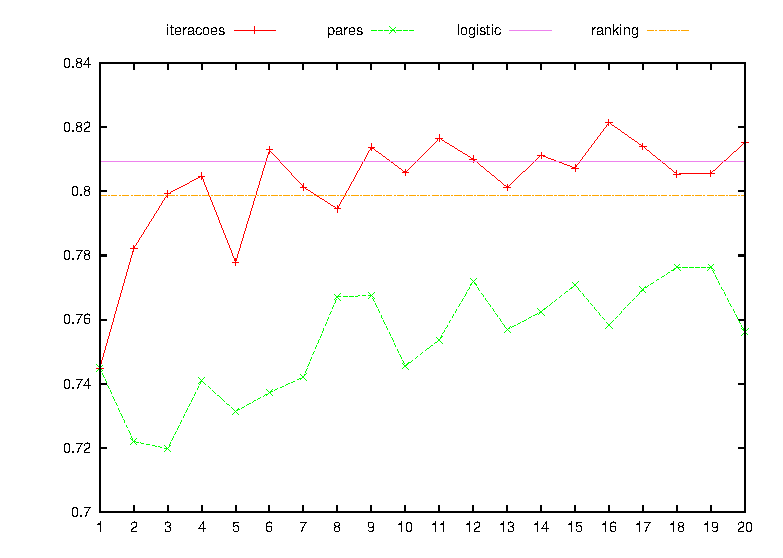
\includegraphics[width=0.42\textwidth]{img/hepatitis_logistic.eps}
    }    
    \subfloat[Vehicle]{
        \label{fig:vehicle_logistic}
        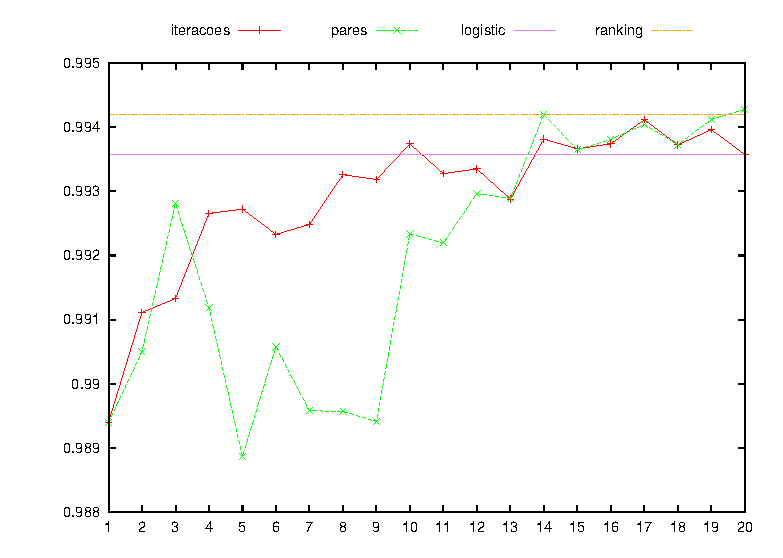
\includegraphics[width=0.42\textwidth]{img/vehicle_logistic.eps}
    }

    \subfloat[Yeast]{
        \label{fig:yeast_logistic}
        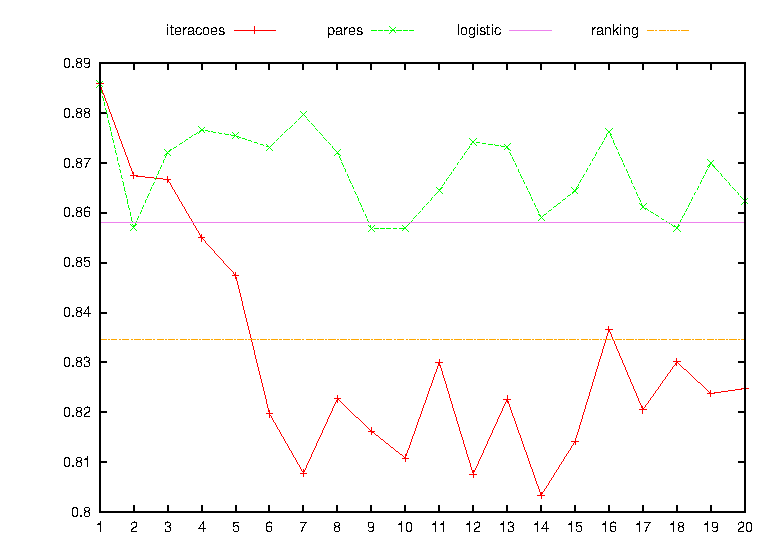
\includegraphics[width=0.42\textwidth]{img/yeast_logistic.eps}
    }

    \caption{Gráficos de desempenho para Curva Logística}
\end{figure}

\clearpage
\pagebreak


\subsection{Desempenho para \emph{Support Vector Machine} (functions.SMO)}

\begin{table}[h!]
    \begin{tabular}{ c c c c c }
        \hline

        \multirow{2}{*}{Bases} & \multirow{2}{*}{SMO} & \multicolumn{3}{c}{SMO acrescido de} \\ \cline{3-5}
        & & {\small Ranking Original} & {\small Ranking*} & {\small  Ranking**} \\
        
        \hline
        
        breast-cancer & {\small 0,59272 (0,00696)} & {\small \textbf{0,66670 (0,02294)}} & {\small 0,65832 (0,02119)} & {\small 0,65563 (0,02003)} \\
        vehicle & {\small 0,94434 (0,00169)} & {\small \textbf{0,99651 (0,00001)}} & {\small 0,99396 (0,00002)} & {\small 0,99380 (0,00002)} \\
        hepatitis & {\small 0,75128 (0,01618)} & {\small \textbf{0,81522 (0,01914)}} & {\small 0,80759 (0,01899)} & {\small 0,78189 (0,02640)} \\
        glass & {\small 0,89181 (0,00679)} & {\small \textbf{0,95712 (0,00175)}} & {\small 0,93402 (0,00610)} & {\small 0,93752 (0,00537)} \\
        yeast & {\small 0,77391 (0,04799)} & {\small 0,83555 (0,04831)} & {\small \textbf{0,99891 (0,00001)}} & {\small \textbf{0,99891 (0,00001)}} \\
    
        \hline
    \end{tabular}
    
    \caption{Desempenho para Support Vector Machine}
    \label{smo_results_table}
\end{table}

\begin{figure}[h!]
    \centering
    \subfloat[Breast cancer]{
        \label{fig:breast-cancer_smo}
        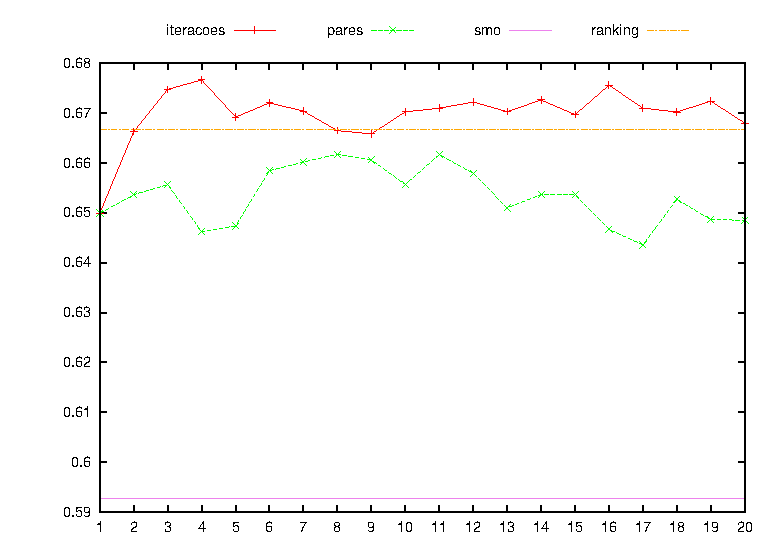
\includegraphics[width=0.42\textwidth]{img/breast-cancer_smo.eps}
    }
    \subfloat[Glass]{
        \label{fig:glass_smo}
        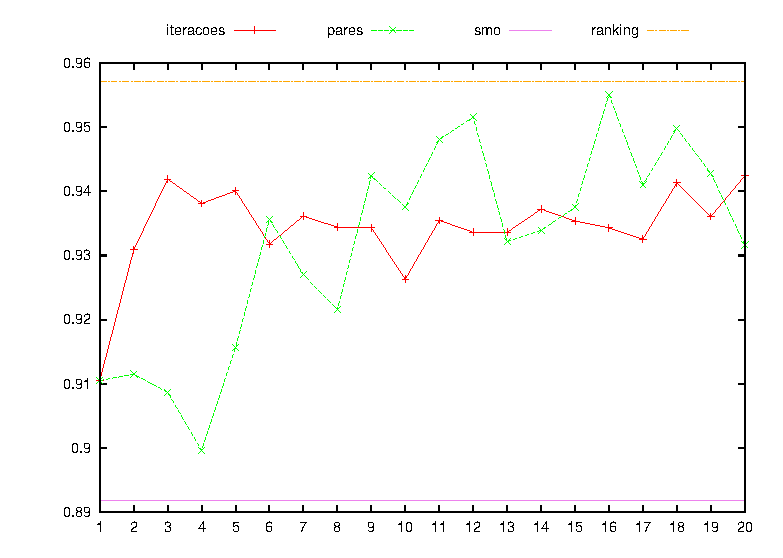
\includegraphics[width=0.42\textwidth]{img/glass_smo.eps}
    }

    \subfloat[Hepatitis]{
        \label{fig:hepatitis_smo}
        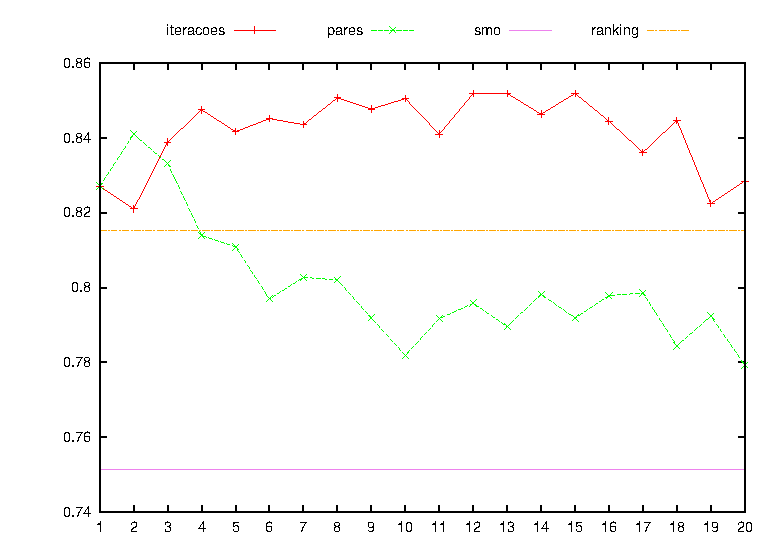
\includegraphics[width=0.42\textwidth]{img/hepatitis_smo.eps}
    }    
    \subfloat[Vehicle]{
        \label{fig:vehicle_smo}
        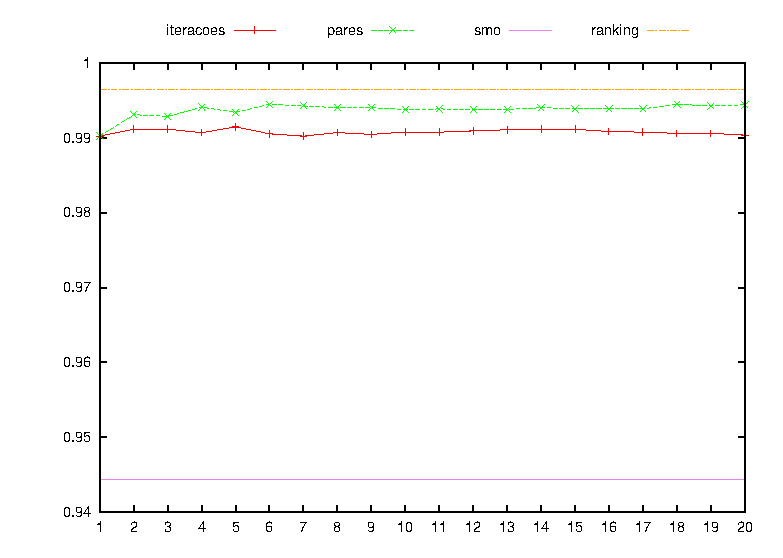
\includegraphics[width=0.42\textwidth]{img/vehicle_smo.eps}
    }

    \subfloat[Yeast]{
        \label{fig:yeast_smo}
        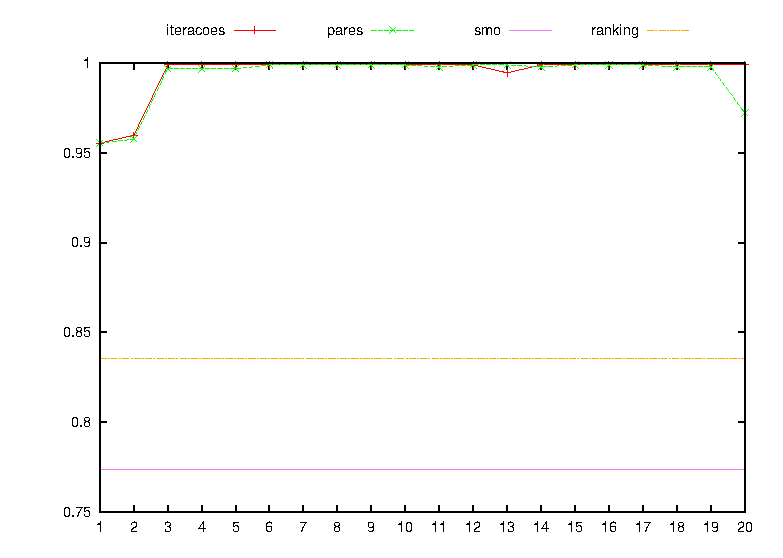
\includegraphics[width=0.42\textwidth]{img/yeast_smo.eps}
    }

    \caption{Gráficos de desempenho para Support Vector Machine}
\end{figure}